\documentclass{automatextcc}
\usepackage{graphicx} % Para importar figuras
\usepackage{float} % Para posicionar as figuras de forma mais conveniente
\graphicspath{{Imagens/}}

\begin{document}

%título do trabalho
\title{Acelerando operações filogenéticas usando programação paralela}
%autor do trabalho
\author{Thiago Pereira Maia dos Santos}
%orientador(a) do trabalho {nome}{Orientador(a)}
\advisor{Prof. Wellington Santos Martins}{Orientador}
%universidade onde obteve o título e atual

\advisorinfo{Doutor pela \ufrgs~--~ Goiânia, GO}{UFG}
%outro exemplo
%\advisor{Prof. Dr. Heraldo José de Amorim}{Orientador}
%\advisorinfo{Doutor pela \ufrgs~--~Porto Alegre, RS}{UFRGS}
%banca examinadora:
\examinera{Prof. Dr. xxx}
\examinerainfo{Doutor pela Universidade Federal de Santa Catarina -- Florianópolis, SC}{UFRGS}
\examinerb{Prof. Dr. xxx}
\examinerbinfo{Doutor pela \ufrgs~-- Porto Alegre, RS}{UFRGS}
\examinerc{Prof. Dr. xxx}
\examinercinfo{Doutor pela \ufrgs~-- Porto Alegre, Rs}{UFRGS}
%departamento:
\dept{\DELAE}
%\dept{\DEMEC}
%\dept{|DELET}
%data de entrega
\date{Julho de 2017}
%cria a capa

\maketitle

%agradecimentos
\chapter*{Agradecimentos}
Agradeço a xxx.
%palavras chave - português
\keyword{Controle de qqq}
\keyword{yyy}
\keyword{zzz}
\keyword{zzz}
%palavras chave- inglês
\keyworde{aaa}
\keyworde{bbb}
\keyworde{ccc}
\keyworde{ddd}
%resumo
\begin{abstract}
Este trabalho ....
\end{abstract}
%abstract
\begin{englishabstract}
This work ....
\end{englishabstract}
%sumário
\tableofcontents
% lista de ilustrações
\listoffigures
% lista de tabelas
\listoftables
% lista de abreviaturas e siglas em ordem alfabética
% o parametro deve ser a abreviatura mais longa
\begin{listofabbrv}{DELAE}
        \item[DELAE] Departamento de Sistemas Elétricos de Automação e Energia
        \item[DELET] Departamento de Engenharia Elétrica
        \item[DEMEC] Departamento de Engenharia Mecânica
        \item[DEQUI] Departamento de Engenharia Química
\end{listofabbrv}
% lista de símbolos em ordem alfabética (opcional)
\begin{listofsymbols}{$\alpha\beta\pi\omega$}
       \item[$\alpha\beta\pi\omega$] variável xxx
       \item[$\sum$] Somatório
\end{listofsymbols}
%%%%%%%%%%%%%%%%%%%%%%%%%%%%%%%%%%%%%%%%%%%%%%%%%%%%%%%%%%%%%%%%%%%%%%%%%%%%%%%%
%COMEÇA O TEXTO DO TRABALHO DE CONCLUSÃO
%%%%%%%%%%%%%%%%%%%%%%%%%%%%%%%%%%%%%%%%%%%%%%%%%%%%%%%%%%%%%%%%%%%%%%%%%%%%%%%%
\chapter{Introdução}
Segundo \cite{Bazanella:GomesdaSilva:2006}. Uma figura pode ser vista na Figura \ref{tanque}. A Tabela \ref{tabela_nota} indica xxx.
\begin{figure}[htb]%
\centering
%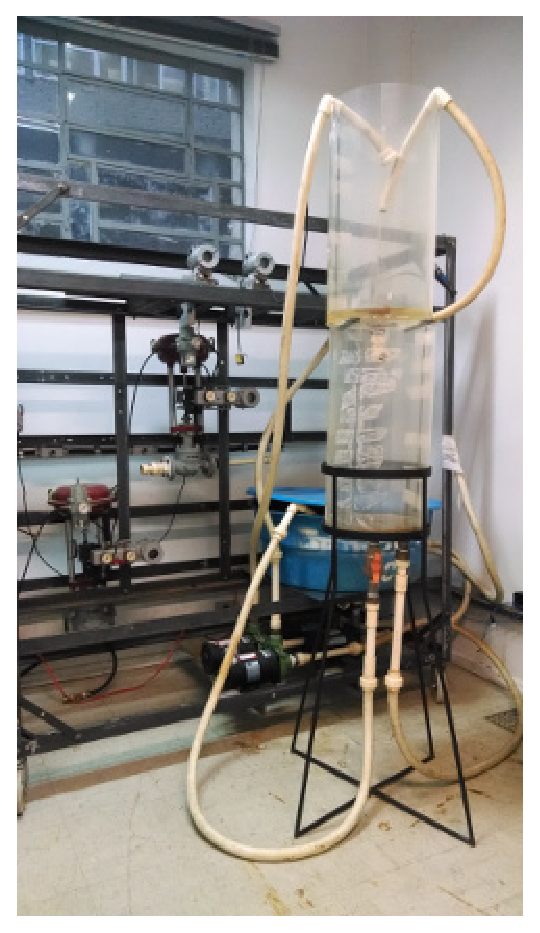
\includegraphics[width=0.5\columnwidth]{tanques}%
\caption{yyy do lab.}%
\label{tanque}%
\end{figure}

\chapter{Desen}
\section{Test}
\begin{table}[htb]%
\centering
\begin{tabular}{|c|c|}
\hline
aaa & bbb\\
\hline
zzz1 & www1\\
\hline
\end{tabular}
\caption{Tabela de xxx}
\label{tabela_nota}
\end{table}
%bibliografia usando o bibtex
%Para se editar a bibliografia deve-se editar o arquivo biblio.bib, que pode ser feito através de um editor padão do latex ou até do bloco de notas(não recomendo).
\bibliographystyle{abnt}
\bibliography{biblio}
\end{document}



